\documentclass{beamer}

\usetheme{Padova}
\usepackage[english, italian]{babel}
\usepackage{float}
\newcommand{\code}[1]{\texttt{#1}}


\title{Integrazione di Single Sign-On in Unix Pluggable Authentication Module (Unix PAM)}
\subtitle{Dipartimento di Matematica ”Tullio Levi-Civita" \\ Università degli Studi di Padova \\ Laurea in Informatica}
\author{Ivan Antonino Arena}
\date{20 luglio 2023}


\begin{document}

	\maketitle

	\begin{frame}{Outline}
		\tableofcontents
	\end{frame}


	\section{Introduzione}
	
	\begin{frame}{L'azienda}
		
		\begin{figure}[H] 
			\centering 
			
\includegraphics[width=0.4\columnwidth]{immagini/logo-athesys} 
			\label{fig:athesys}
		\end{figure}
		
		Ricerca e sviluppo in ambito di sicurezza informatica con Athesys Srl:
		
		\begin{itemize}
			\item Identità digitale \vspace{.5em}
			\item Sistemi di autenticazione \vspace{.5em}
		\end{itemize}
	\end{frame}
	
	
	\begin{frame}{L'azienda}
		\begin{figure}[H] 
			\centering 
			
\includegraphics[width=0.4\columnwidth]{immagini/logo-monokee} 
			\label{fig:monokee}
		\end{figure}


		\begin{itemize}
			\item Identity as a Service \vspace{.5em}
			\item Single Sign-On \vspace{.5em}
			\item Self-Sovereign Identity \vspace{.5em}
		\end{itemize}	
	\end{frame}
	
	\begin{frame}{Il progetto}
		\begin{block}{Obiettivo}
			Ricercare e sviluppare una soluzione che consenta di effettuare l'accesso a Monokee utilizzando il relativo SSO da riga di comando di dispositivi Linux (CentOS e RHEL).
		\end{block}
	\end{frame}
	
	\begin{frame}{Roadmap}
				
		\begin{enumerate}
			\item Studio tecnologico \vspace{.5em}
			\item Ricerca soluzione (PAM/FreeIPA) \vspace{.5em}
			\item Sviluppo PoC \vspace{.5em}
		\end{enumerate}
		
	\end{frame}
	
	\section{Tecnologie utilizzate}
	
	\begin{frame}{Tecnologie utilizzate}
		
		\begin{itemize}
			\item FreeIPA \vspace{.5em}
			\item LXC/Proxmox \vspace{.5em}
			\item Secure Shell (SSH) \vspace{.5em}
		\end{itemize}
		
		\begin{figure}[H] 
			\centering 
			
\includegraphics[width=0.4\columnwidth]{immagini/logo-freeipa.png} 
			\label{fig:freeipa}
		\end{figure}
	\end{frame}
	
	\section{Ricerca e sviluppo}
	
	\begin{frame}{Configurazione dello stato iniziale}
		\begin{figure}[H] 
			\centering 
			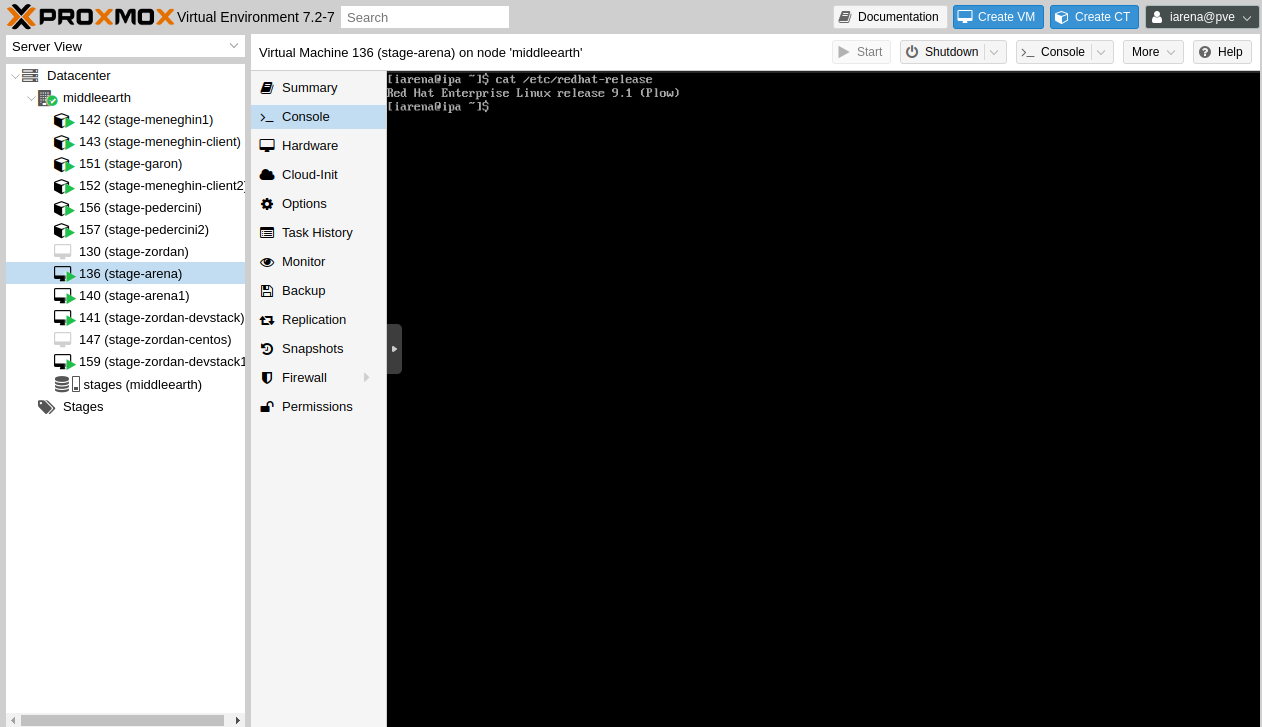
\includegraphics[width=0.6\columnwidth]{immagini/proxmox.png} 
			\label{fig:proxmox}
		\end{figure}
		
		\begin{itemize}
			\item Configurazione macchine CentOS, RHEL e Ubuntu \vspace{.5em}
			\item Installazione FreeIPA \vspace{.5em}
		\end{itemize}
		
	\end{frame}
	
	\begin{frame}{Linux PAM}
				
		\begin{itemize}
			\item Studio documentazione PAM \vspace{.5em}
			\item Realizzazione PoC modulo PAM e app PAM-aware \vspace{.5em}
		\end{itemize}
		
	\end{frame}
	
	\begin{frame}{FreeIPA Identity Provider}
		
		\begin{itemize}
			\item Configurazione OAuth2 e OIDC su Monokee \vspace{.5em}
			\item Configurazione FreeIPA IdP \vspace{.5em}
			\item PoC CLI Monokee SSO \vspace{.5em}
			
			\begin{figure}[H] 
				\centering 
				
\includegraphics[width=0.5\columnwidth]{immagini/oidc_logo.png} 
				\label{fig:oidc-setup}
			\end{figure}
		\end{itemize}
	\end{frame}
	
	% \begin{frame}{OpenID Connect}
	% 	\begin{figure}[H] 
	% 		\centering 
	% 		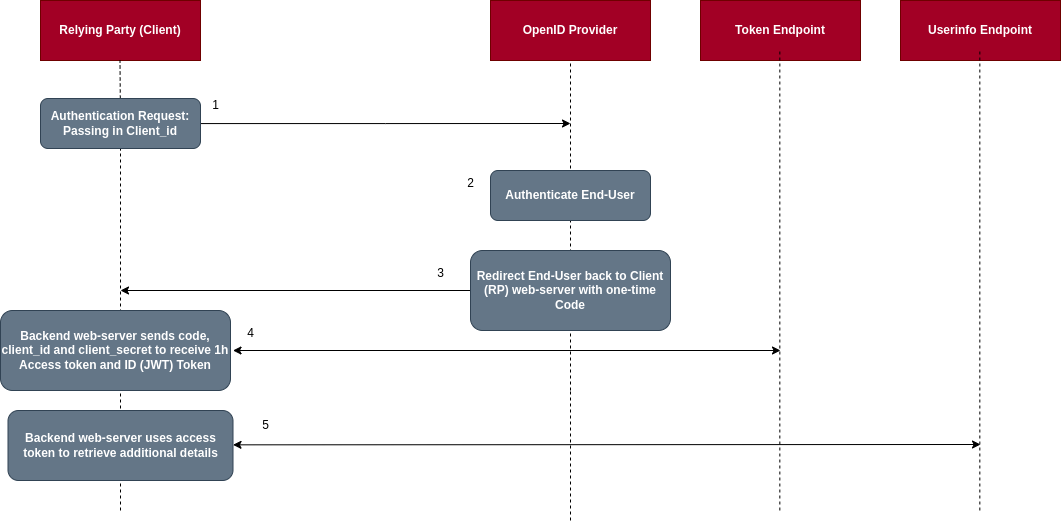
\includegraphics[width=\columnwidth]{immagini/oidc-flow.png} 
	% 		\label{fig:oidc-flow}
	% 	\end{figure}

	% \end{frame}
	
	\begin{frame}{Configurazione OAuth2 e OIDC su Monokee}
		\begin{figure}[H] 
			\centering 
			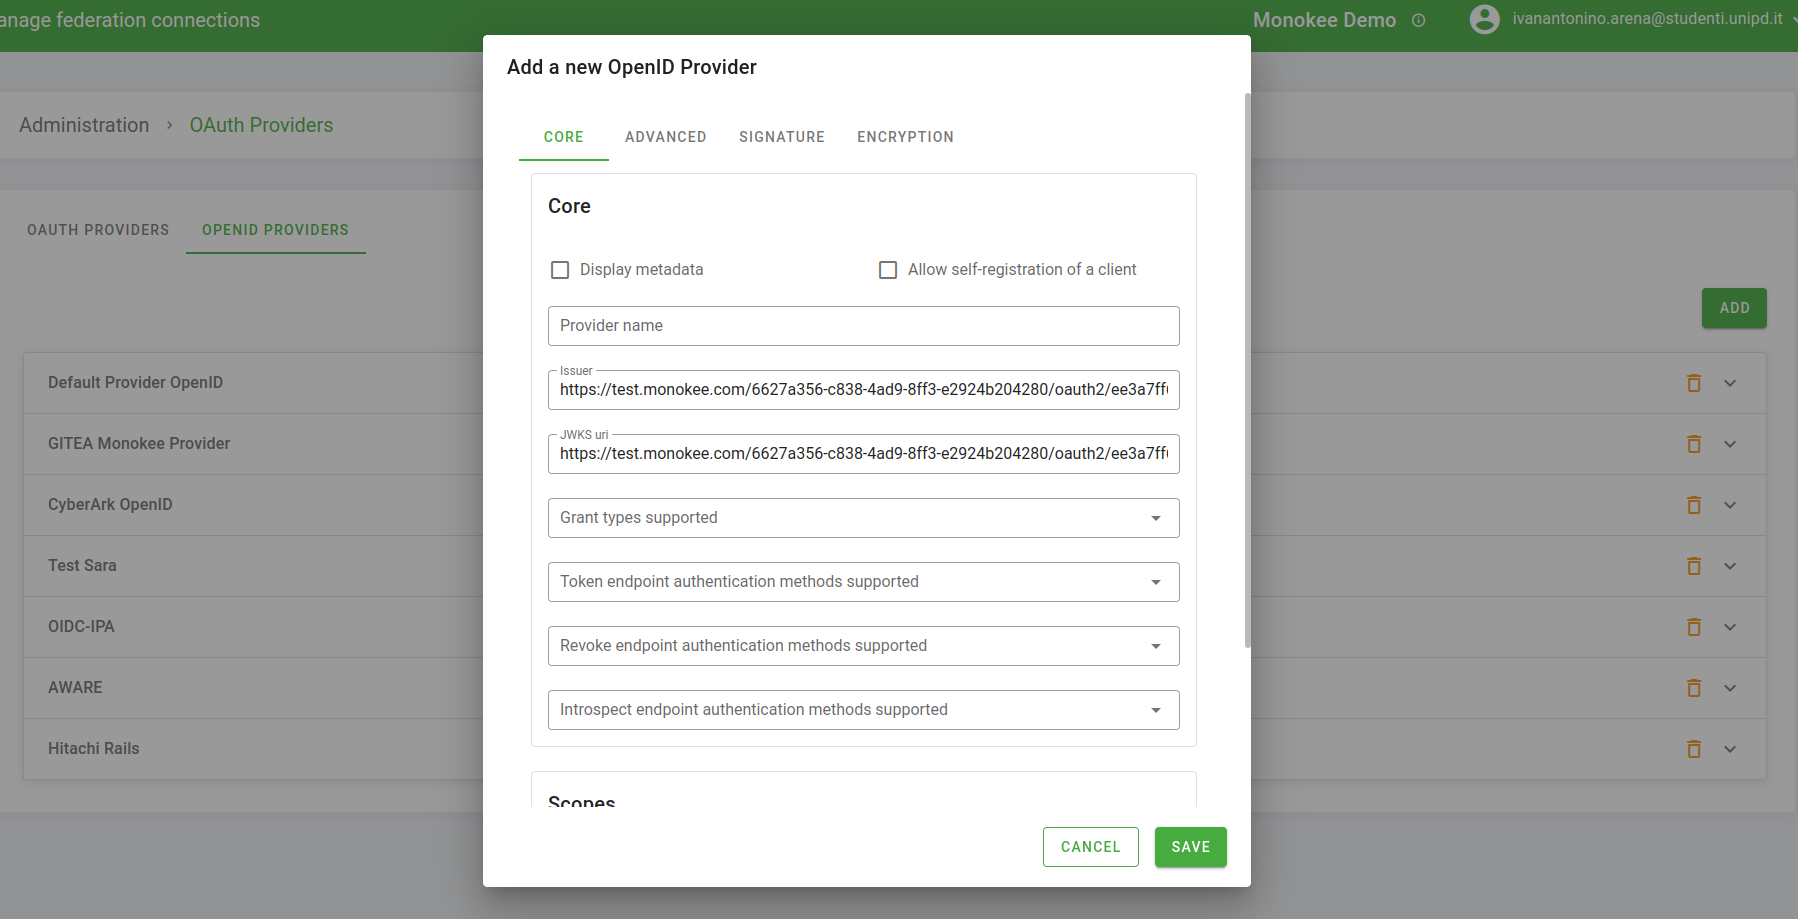
\includegraphics[width=\columnwidth]{immagini/monokee-oidc.png} 
			\label{fig:oidc-setup}
		\end{figure}
		
	\end{frame}
	
	\begin{frame}{Configurazione FreeIPA IdP}
		
		\begin{figure}[H] 
			\centering 
			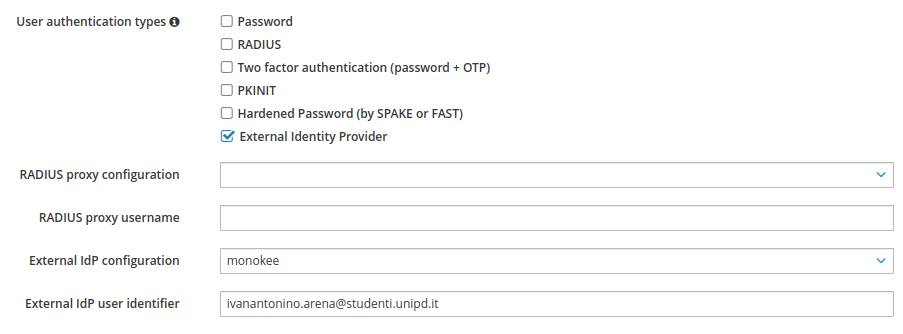
\includegraphics[width=\columnwidth]{immagini/appendici/ipa-user.png} 
			\label{fig:ipa-setup-user}
		\end{figure}
	\end{frame}
	
	\begin{frame}{PoC CLI Monokee SSO}
		\textbf{\textit{Caso d'uso:} un utente registrato vuole operare su una macchina virtuale fornita da Monokee}
		\vspace {.5em}
		\begin{enumerate}
			\item L'utente accede alla macchina virtuale;
			\item L'utente inserisce i comandi per l'autenticazione;
			\item L'utente segue il link fornito e si autentica con il metodo che preferisce;
			\item L'utente ritorna al terminale e preme "Invio";
			\item L'utente è correttamente autenticato e può operare sulla macchina.
		\end{enumerate}
	\end{frame}

	\begin{frame}{PoC CLI Monokee SSO}
		\code{[iarena@ipa]\$ kinit -n -c ./fast.ccache} \\
		\code{[iarena@ipa]\$ kinit -T ./fast.ccache monokee1} \\
		\code{Authenticate at https://test.monokee.com/6627a356/device?user\_code=XYhv-HksZ and press ENTER.:} \\
		\code{[iarena@ipa]\$ klist}
	\end{frame}
	\begin{frame}{Stato dello sviluppo}
				
		\begin{exampleblock}{Stato attuale}
			\begin{itemize}
				\item SSO Monokee (implementato con FreeIPA) \vspace{.5em}
				\item Documentazione (in formato Markdown) \vspace{.5em}
			\end{itemize}
		\end{exampleblock}
		
		\begin{block}{Sviluppi futuri}
			Accesso da remoto (SSH) ai dispositivi Linux con FreeIPA e Monokee SSO implementato.
		\end{block}
	
	\end{frame}
	
	

	\section{Conclusioni}
	\begin{frame}{Conclusioni}
		
		\begin{exampleblock}{Obiettivi raggiunti}
			Implementato l'SSO Monokee da terminale Linux.
		\end{exampleblock}
				
		\vspace{.5em} \textbf{Conoscenze acquisite:} \vspace{.5em}
		\begin{itemize}
			\item Migliorata conoscenza degli ambienti Linux \vspace{.5em}
			\item Concetti di SSO e SSI \vspace{.5em}
			\item Protocolli moderni di autenticazione e autorizzazione \vspace{.5em}
		\end{itemize}
	
	\end{frame}
	
	\begin{frame}{Conclusioni}
		
		Grazie per l'attenzione.
	
	\end{frame}
	\section{Note bigliografiche}



	% EXAMPLE BLOCKS ---------------------------------------------
	% \begin{frame}{L'azienda}
	% 	\begin{block}{Normal block}
	% 		Fusce luctus venenatis felis quis semper
	% 	\end{block}

	% 	\begin{alertblock}{Alert block}
	% 		$$ E = (x_1 \vee \neg x_2 \vee \neg x_3) \wedge (x_1 \vee x_2 \vee x_4) $$
	% 	\end{alertblock}

	% 	\begin{exampleblock}{Example block}
	% 		Proin tincidunt, neque at tincidunt mollis
	% 	\end{exampleblock}
	% \end{frame}


\end{document}
